% !TEX program = xelatex

% Joint Programme with University of Information Technology, VNU-HCM
% Module: Individual Honours Project
%
% -----
%
% A Game-Based Approach to Motor Imagery Adaptation and BCI Calibration
% Author: Cao Đăng Khoa (dang.cao@mail.bcu.ac.uk)
% Student ID: 25195675
%
% Supervisor: Dr. Vi Chí Thành (vcthanh@hcmiu.edu.vn)
%------------------------------------%



%------ DOCUMENT CONFIGURATION ------%
\documentclass[a4paper, 11pt, openany]{report}
\usepackage{layout}
\usepackage{fonts}
\usepackage{headerfooter}
\usepackage{frontmatter}
\usepackage{contents}
\usepackage{atbegshi}
\usepackage[round, authoryear]{natbib}
\usepackage{graphicx}
\usepackage{booktabs}
\usepackage{array}


% Make \cite produce (Author, Year)
\let\cite\citep

\makeatletter
\let\ps@plain\ps@fancy
\makeatother


%------------------------------------%



%----------- FRONT MATTER -----------%
\begin{document}

% Title Page
\reportTitlePage
    {Project Interim Report}
    {BCG: A Game-Based Approach to Motor Imagery Adaptation and BCI Calibration}
    {Cao Đăng Khoa}{25195675}
    {Bachelor of Science with Honours Computer Science}
    {Dr. Vi Chí Thành}{December 8, 2025}
    \thispagestyle{titlepage}

% Page numbering
\pagenumbering{roman}
\setcounter{page}{0}

% Table of Contents
\reportTableOfContents

% List of Figures
\reportListOfFigures

% List of Tables
\reportListOfTables
%------------------------------------%


\cleardoublepage
\pagenumbering{arabic}

\setstretch{1.2} 
\setlength{\parskip}{8pt plus 2pt minus 1pt} 


%------------ CHAPTER 1 -------------%
%----- Introduction and Context -----%
\vspace*{-1.15cm}
\chapter{INTRODUCTION AND CONTEXT}

    % 1.1 Background and Significance
    \section{Background and Significance}

    The way humans interact with computers has undergone a significant evolution over time. 
    From early keyboards and mice to modern touchscreen devices and voice assistants, 
    each innovation has expanded how people can engage with digital systems. But what 
    if humans were able to communicate with technology simply by thought? This is what 
    next-generation technology is achieving: Brain-Computer Interfaces (BCIs), systems 
    that allow people to control devices with their thoughts \cite{Birbaumer2006}. By 
    reading neural signals directly from the human brain and translating them into 
    digital commands for computers to understand, BCIs not only enhance the experience 
    for typical users but also enable people with physical limitations to access technology 
    more easily.

    Among various types of BCI applications, electroencephalography-based motor imagery 
    (EEG-MI) is one of the most widely studied areas \cite{Lotte2018}. This concept is 
    based on a key principle of neuroscience: whenever a person imagines a movement,
    such as moving a hand or foot, without performing it physically, their brain still 
    produces characteristic signals with patterns that are remarkably similar to the 
    actual physical execution \cite{Neuper2001}. Building on this principle, EEG-based 
    MI has been applied in many real-world scenarios, including motor rehabilitation, 
    assistive control for individuals with disabilities, and control of games
    \cite{pfurtscheller1999event}.

    These promising applications, however, still depend heavily on how accurately MI 
    signals can be detected. This accuracy is influenced by many factors, with the 
    calibration process playing a crucial role, which is also the 
    main focus of this project \cite{Lotte2018}.


    % 1.2 Current State and Limitations
    \section{Current State and Limitations}

    In controlled laboratory environments, where the calibration process is managed 
    with precision, EEG-MI systems demonstrate a high level of performance in classifying 
    motor signals \cite{Lotte2018}. After an initial training phase, these classifiers 
    often reach accuracies above 70\% in distinguishing between imagined movements such 
    as left hand, right hand, foot, or a rest state, a level that is commonly taken as 
    the threshold for effective BCI control \cite{Kübler2001}.

    However, achieving this level of performance for each individual user requires a 
    significant calibration effort. In practice, the system must learn a user's specific
    neural patterns through 15-30 minutes of supervised training, typically collecting
    40-80 labelled trials per movement class, around 120-240 trials in total \cite{Giles2022}. 
    Moreover, these EEG patterns vary significantly between sessions even for the same 
    user due to non-stationarities \cite{Sugiyama2008}.

    The repetitive and cognitively demanding nature of EEG-MI makes it challenging to 
    implement outside controlled laboratory settings \cite{Xu2024}. It is time-consuming, 
    requires dedicated human supervision, and depends on specialised lab facilities - which are
    often geographically distant. It also induces cognitive fatigue, degrades signal 
    quality over time, and limits practicality for multi-session applications like 
    rehabilitation \cite{Xu2024}. Consequently, despite decades of research, this 
    technology remains largely confined to laboratories rather than achieving 
    widespread real-world adoption \cite{Wolpaw2002}.


    % 1.3 Problem Statement
    \section{Problem Statement}

    EEG-MI calibration per session requires 15-30 minutes of repetitive trials, which limits 
    real-world scalability despite over 70\% success in the experimental environment 
    \cite{Giles2022,Kueper2024}. This limitation arises from changes in brain signals 
    between sessions and across different individuals \cite{Sugiyama2008}, the need for 
    human supervision \cite{Giles2022}, and reliance on specific infrastructure \cite{Lotte2018}.


%------------------------------------%

%------------ CHAPTER 2 -------------%
%--- Review of Existing Knowledge ---%


\chapter{REVIEW OF EXISTING KNOWLEDGE}

    % 2.1 The Neuroscience of Motor Imagery
    \section{The Neuroscience of Motor Imagery}
    To interpret human intention, we must examine the concept of functional 
    equivalence. Modern research has shown that planning a movement and 
    physically performing it are not distinct processes \cite{Jeannerod1995}. 
    When a person performs Motor Imagery, mentally imagining a movement while 
    remaining physically still, their brain activates many of the same neural 
    networks used during actual execution.

    When a user imagines moving a limb, such as their right hand, the primary 
    motor cortex generates specific, rhythmic electrical patterns. These patterns 
    occur in the sensorimotor cortex and are governed by the contralateral 
    principle: imagining a right-hand movement primarily activates the left 
    hemisphere, while left-hand imagery activates the right \cite{Wolpaw2002}.

    These activations are measurable through changes in brain rhythms. In a 
    resting state, neurons fire in synchrony, creating strong idle rhythms known 
    as Mu (8-13 Hz) and Beta (13-30 Hz). When the user begins imagining movement, 
    this synchrony is disrupted, causing a power drop known as Event-Related 
    Desynchronisation (ERD). Conversely, when the brain relaxes, the neurons 
    synchronise again, leading to Event-Related Synchronisation (ERS) \cite{Pfurtscheller2001}.

    These ERD/ERS patterns are the core signatures BCI systems are trained to 
    recognise. While they are highly reproducible and occur even in individuals 
    with severe motor disabilities, their specific structure varies significantly 
    between individuals \cite{Lotte2018}. The frequency and spatial distribution 
    of these signals are unique to each person, necessitating a system that can 
    adapt to the user.
    
    \begin{figure}[h]
    \centering
    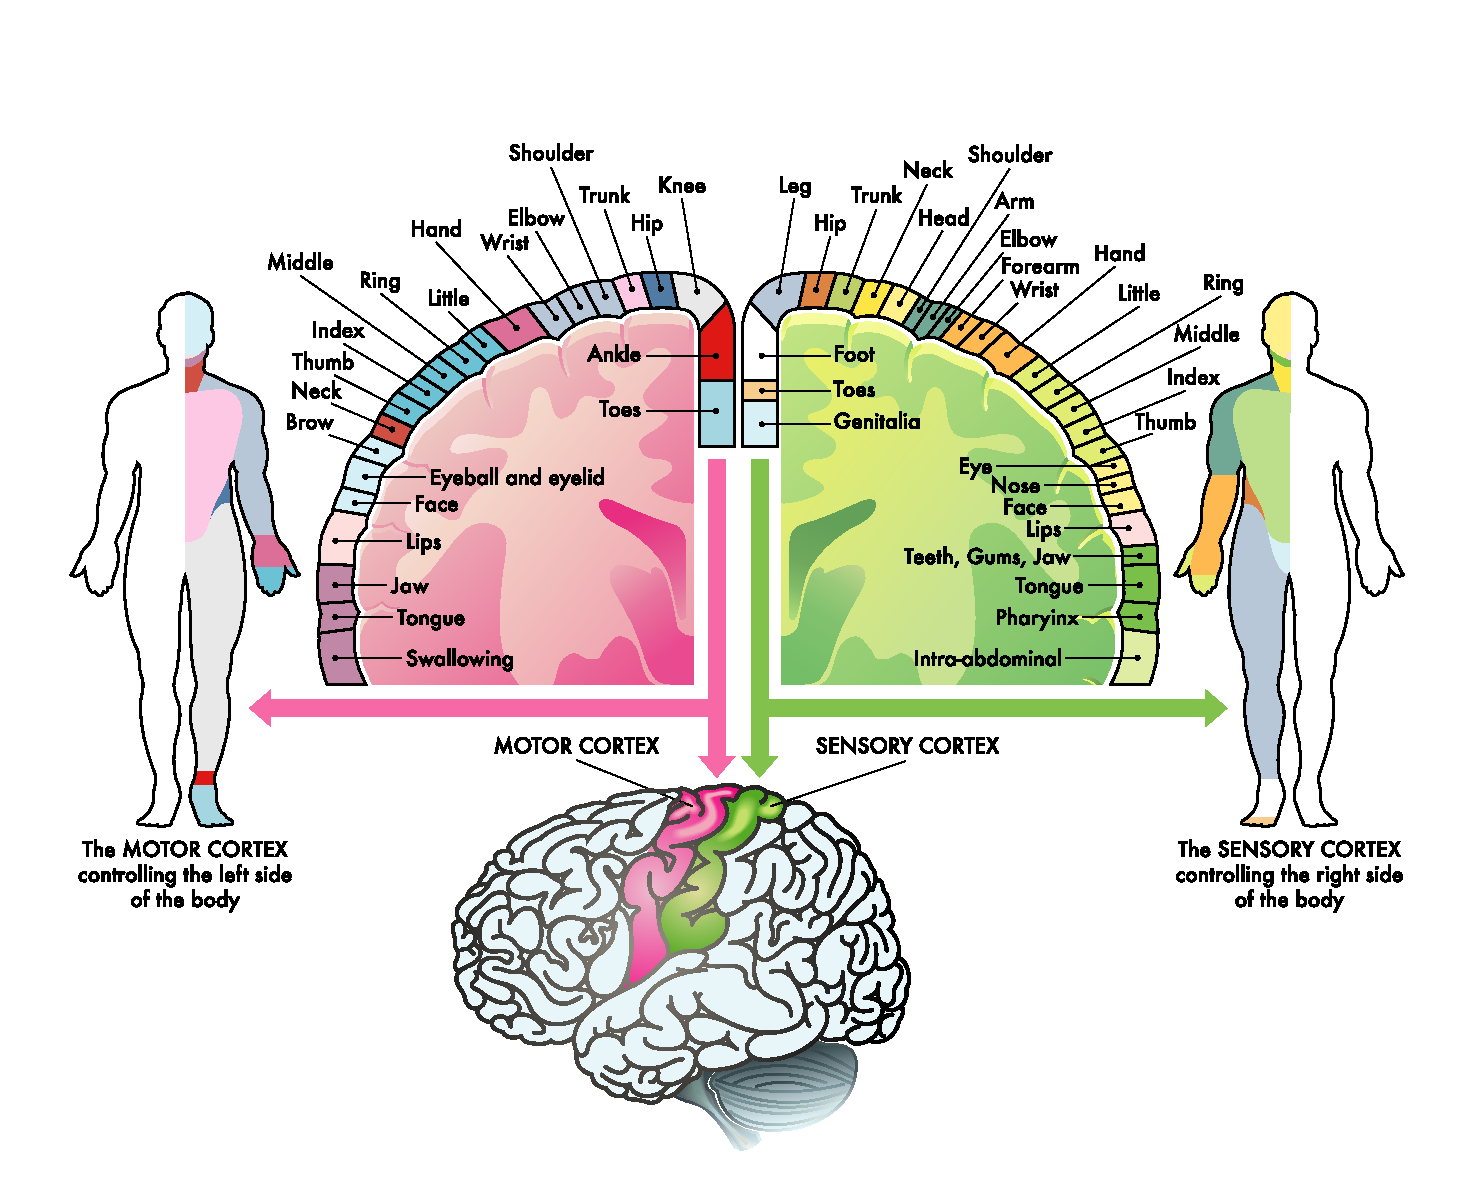
\includegraphics[width=1\textwidth]{Images/neuroscience-of-motor-imagery.pdf}
    \caption{Motor Cortex Organization and Contralateral Hemispheric Control}
    \label{fig:neuroscience-of-motor-imagery}
    \end{figure}

    % 2.2 The EEG Processing Pipeline
    \section{The EEG Processing Pipeline}
    Capturing these neural signatures non-invasively is a significant engineering 
    challenge. Raw scalp EEG is weak, often in the microvolt range, and obscured 
    by noise such as muscle movement and electrical interference \cite{Niedermeyer2004}. 
    Therefore, data must pass through a strict processing pipeline.

    The first stage is preprocessing. Since motor imagery activity is concentrated 
    in the Mu and Beta bands (8-30 Hz), bandpass filters are applied to isolate 
    these frequencies, removing high-frequency muscle noise and slow baseline 
    drifts. Following this, spatial filtering is used to boost the signal-to-noise 
    ratio. This mathematically separates mixed signals from multiple electrodes, 
    isolating activity from the sensorimotor cortex while suppressing noise from 
    unrelated brain regions.
  
    The next stage is feature extraction. The well-known algorithm for 
    this is Common Spatial Patterns (CSP) \cite{Blankertz2008}. CSP functions 
    like a sophisticated filter that combines signals from different electrodes 
    to create new channels. Its goal is to find a specific blend that maximises 
    the variance of signal power for one task (e.g., right hand) while minimising 
    it for another. This transforms complex biological signals into separable 
    features, simplifying the prediction task for the computer.


    % 2.3 Classification Strategies
    \section{Classification Strategies}
    Once features are extracted, they are fed into a classifier to determine the 
    user's intent. For years, Linear Discriminant Analysis (LDA) and Support 
    Vector Machines (SVM) have been the standard classifiers \cite{Lotte2018}. 
    They remain popular due to their computational efficiency on small datasets, 
    making them ideal for real-time applications.

    Recently, the field has explored Deep Learning techniques, such as 
    Convolutional Neural Networks (CNNs) \cite{Raza2019}. These models promise 
    to automatically learn features from raw data, potentially bypassing manual 
    steps like CSP. However, Deep Learning models typically require thousands 
    of trials to perform reliably \cite{Roy2019}. This is often impractical 
    for real-time BCI usage, where setup time must be minimised. Therefore, 
    traditional pipelines using CSP and LDA remain the most practical choice 
    for achieving high accuracy with limited calibration time.


    % 2.4 The Calibration Bottleneck
    \section{The Calibration Bottleneck}
    Despite advanced algorithms, a significant obstacle prevents widespread 
    adoption: the dependency on long and repetitive calibration. Current 
    high-performing BCI systems typically use the ``Standard Graz Protocol'', 
    where the user follows a fixed sequence of abstract prompts (e.g., arrows 
    on a screen) for 20 to 30 minutes \cite{Pfurtscheller2001}.

    This phase is compulsory because brain signals are non-stationary. They 
    change constantly due to fatigue, attention levels, and electrode shifts \cite{Sugiyama2008}. 
    A classifier trained on Monday could fail on Tuesday because the statistical 
    distribution of the data has shifted. Consequently, the system must 
    essentially re-learn the user at the start of every session.

    This process creates a severe bottleneck. The abstract nature of the protocol 
    induces boredom and cognitive fatigue \cite{Xu2024}. As the user tires, 
    their ability to generate distinct neural patterns degrades, leading to 
    poor quality data. This creates a cycle where poor data leads to a poor 
    classifier, frustrating the user and further degrading signal quality.


    % 2.5 Gamification in BCI
    \section{Gamification in BCI}
    Gamification applies game-design elements to non-game contexts to enhance 
    motivation. In BCI, this is typically utilised during Neurofeedback training \cite{Skola2019}. 
    Instead of abstract cues, users interact with compelling elements, such as 
    controlling a race car. Research confirms that this approach improves signal 
    quality; when a user is motivated and enters a flow state, their attention 
    focuses, producing more pronounced ERD/ERS patterns \cite{Atilla2024}.

    However, the application of gamification remains uneven. While the training
    phase has evolved, the critical calibration phase often retains rigid, 
    repetitive protocols. Users must endure a fatiguing setup before accessing the 
    engaging interface, leading to a loss of engagement exactly when the system 
    needs high-quality data.

    This presents a significant opportunity: by applying engagement mechanics 
    directly to the calibration phase, it is theoretically possible to collect 
    high-quality data. This would transform calibration from a 
    tedious setup barrier into a seamless part of the user experience. However, 
    the game design process is critical. If a game is visually chaotic, it may 
    generate interfering signals. The design must balance engagement with signal purity.


    % 2.6 Critical Analysis and Project Justification
    \section{Critical Analysis and Project Justification}
    This review reveals a contradiction in BCI research: theoretical foundations 
    are strong, but practical application is limited by the calibration bottleneck. 
    Mathematical solutions like Transfer Learning address the lack of data but
    struggle with biological non-stationarity \cite{Sugiyama2008}. Conversely, 
    gamification improves signal quality but is rarely applied to the calibration 
    phase itself.

    Therefore, a significant gap exists: there is a lack of frameworks 
    that replace the standard, repetitive calibration protocol with an engaging, 
    game-based alternative.

    This project directly addresses this gap. By developing a system that uses a 
    game as the data collection task, this project aims to investigate 
    whether a Gamified Calibration Protocol (playing to calibrate) can 
    effectively replace the traditional Standard Graz Protocol. If successful, 
    it will demonstrate that high-quality calibration data can be collected more 
    efficiently while significantly reducing user boredom and cognitive fatigue.

% ------------------------------------%

%------------- CHAPTER 3 -------------%–
%-Project Aims, Objectives, and Scope-%
\chapter{PROJECT AIMS, OBJECTIVES, AND SCOPE}   

    % 3.1 Project Aim
    \section{Project Aim}    
    The primary aim of this project is to investigate and validate the effectiveness 
    of a gamified calibration protocol compared to the standard clinical approach. 
    Specifically, the project seeks to determine if a game-based interface can 
    reduce user cognitive fatigue and perceived setup time while maintaining 
    sufficient signal quality for BCI control.

    % 3.2 Project Objectives    
    \section{Project Objectives}    
    To achieve this aim, the project focuses on the following measurable objectives, 
    prioritised by their contribution to the comparative study:
    
    \begin{enumerate}
        \item \textbf{Framework Development:} Design and implement a dual-mode 
        BCI software framework that supports two distinct data collection protocols:
        \begin{itemize}
            \item \textbf{Condition A (Standard):} A baseline mode replicating the traditional Graz protocol.
            \item \textbf{Condition B (Gamified):} A proposed mode where calibration data is collected implicitly during gameplay.
        \end{itemize}
        
        \item \textbf{User Experience Evaluation:} Conduct a comparative user study 
        to quantitatively assess the psychological impact of the two protocols. 
        The objective is to measure differences in subjective workload 
        (via NASA-TLX) and boredom levels to determine if the gamified 
        approach effectively mitigates calibration fatigue.
        
        \item \textbf{Signal Quality Assessment:} Record and analyse EEG data 
        from both conditions to ensure the gamified approach does not compromise 
        technical performance. The objective is to verify that motor imagery 
        signals (ERD/ERS patterns) generated during gameplay are distinguishable 
        and comparable in quality to those generated during standard training.
        
        \item \textbf{Adaptive Implementation:} Develop and integrate an 
        automatic classifier update mechanism within the game loop. 
        This objective focuses on the technical feasibility of retraining the 
        machine learning model (CSP+LDA) in the background using the labeled 
        game data.
    \end{enumerate}
        
    % 3.3 Project Scope    
    \section{Project Scope}    
    The project boundaries are defined to ensure the feasibility of the 
    comparative study within the academic timeline.
    
    \textbf{In-Scope:}
    \begin{itemize}
        \item Development of the Python-based signal processing backend (preprocessing, feature extraction).
        \item Design of a 2D/3D game environment (e.g., GameMaker or PyGame) specifically for Motor Imagery tasks.
        \item Integration with commercially available dry-electrode headsets (e.g., BrainBit).
        \item Statistical analysis of user fatigue metrics and classification accuracy.
    \end{itemize}
    
    \textbf{Out-of-Scope:}
    \begin{itemize}
        \item Hardware engineering (no sensor modification or headset construction).
        \item Advanced Deep Learning models (focus remains on CSP+LDA for real-time feasibility).
        \item Clinical trials with patients (focus is on healthy user validation).
        \item Long-term adaptation studies (focus is on single-session immediate effects).
    \end{itemize}

%------------- CHAPTER 4 -------------%
%----------- PRODUCT DESIGN -----------%
\chapter{PRODUCT DESIGN}

    % 4.1 Design and Methods
    \section{Design and Methods}
    The project follows an experimental systems development approach, structured 
    to facilitate the direct comparison of the two calibration methods.

    \subsection{Phase 1: System Development}
    The software architecture follows a modular design strategy, prioritizing 
    the development of the core comparative framework. This ensures that the 
    primary objective - validating the user experience differences - is achieved 
    early, with advanced adaptive algorithms integrated as a subsequent layer.
    
    The system is built in three main parts. The first two parts form the 
    foundation, while the third part introduces the advanced intelligence 
    needed to automate the calibration.

    First, we build the Signal Processing Unit. This Python software 
    connects to the EEG headset and captures the raw brain data. Since raw 
    signals are noisy, this unit applies digital filters (8–30Hz) to strip 
    away muscle noise and electrical interference, ensuring the system receives 
    clean motor imagery signals regardless of which calibration mode is active.
    
    Second, we create the Game Interface. This will be a simple continuous 
    game, such as an infinite runner. The game acts as the data collector. 
    When an obstacle appears (e.g., a rock on the left), it makes the user 
    to imagine a movement. This game event creates a natural ``time-stamp'' that 
    tells the system exactly when the user was thinking about moving.
    
    Third, we implement the Adaptive Learning Layer, which is the 
    advanced component of the system. Unlike basic BCI games that just read 
    signals, this smart module runs in the background to analyse the labeled 
    data segments from the game. It uses this data to mathematically retrain 
    the computer instantly, allowing the system to adapt to the user's unique 
    brain patterns automatically without stopping the gameplay.

    \subsection{Phase 2: User Evaluation}
    The validation phase is the core of the project. We will invite healthy 
    participants ($N=5-10$) to test the system in a Within-Subjects experiment.
    
    Each participant will perform two sessions:
    \begin{enumerate}
        \item \textbf{Session A (Traditional-shortened):} The user performs 5 minutes of standard training (watching arrows).
        \item \textbf{Session B (Traditional-standard):} The user performs 15 minutes of standard training (watching arrows).
        \item \textbf{Session C (Gamified):} The user plays the game for 5 minutes.
    \end{enumerate}
    
    By comparing the setup time, accuracy, and reported fatigue 
    between these three sessions, we can validate the project's aim even if the 
    adaptive algorithm requires further refinement.

    % 4.2 Justification of Methods
    \section{Justification of Methods}
    The comparative design is chosen to directly measure the ``Human Factor'' 
    benefits of the system. While technical accuracy is important, the primary 
    argument of this thesis is that gamification reduces the barrier to entry. 
    Therefore, measuring Subjective Workload (NASA-TLX) is just as critical 
    as measuring classifier accuracy. 
    
    Technically, Common Spatial Patterns (CSP) and Linear Discriminant Analysis 
    (LDA) are selected because they are well-documented and computationally 
    light. This minimises the risk of technical failure during the implementation 
    phase, ensuring the requirements are suitable for an individual project.

    % 4.3 Project Timeline
    \section{Project Timeline}

    \begin{figure}[h]
        \centering
        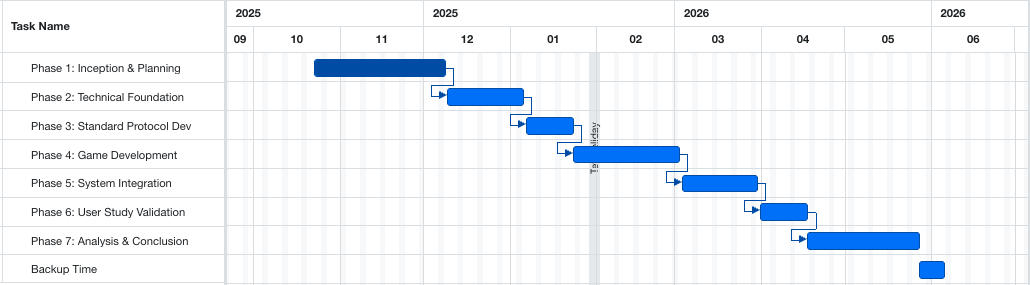
\includegraphics[width=1\textwidth]{Images/timeline.png}
        \caption{Project Timeline}
        \label{fig:timeline}
    \end{figure}

%------------------------------------%



%------------- CHAPTER 5 -------------%
%--- FEASIBILITY, RISKS, & ETHICS ----%
\chapter{FEASIBILITY, RISKS, AND ETHICAL CONSIDERATIONS}

    % 5.1 Feasibility and Resources
    \section{Feasibility and Resources}
    
    \subsection{Project Feasibility}
    This project is assessed as highly feasible. By structuring the work around 
    a comparative framework first, the project ensures a valid research outcome 
    (the comparison of user experience) even if the complexity of real-time 
    adaptation presents challenges. The feasibility is further supported by the 
    use of mature Python libraries and the modular design of the software.

    \subsection{Required Resources}
        The project requires the following resources to ensure successful execution:
        
        \begin{itemize}
            \item \textbf{Hardware:} 
            \begin{itemize}
                \item A 4-channel dry-electrode EEG headband (e.g., BrainBit) with Bluetooth Low Energy (BLE).
                \item A standard development laptop with sufficient processing power for real-time streaming.
            \end{itemize}

            \item \textbf{Software:} 
            \begin{itemize}
                \item \textbf{Development:} Python 3.9+ and libraries (e.g., MNE-Python, Scikit-learn).
                \item \textbf{Game Engine:} GameMaker or PyGame.
                \item \textbf{Version Control:} GitHub will be used for source code management and backup.
                \item \textbf{Analysis:} Statistical software (e.g., SPSS or Excel) for evaluating user study results.
            \end{itemize}

            \item \textbf{Infrastructure \& Environment:} 
            \begin{itemize}
                \item \textbf{Testing Environment:} A quiet, isolated room to minimize external signal artefacts and distraction during data collection.
                \item \textbf{Storage:} Access to University One Drive and secure servers for ethical data management.
            \end{itemize}
        \end{itemize}

% 5.2 Risks and Mitigation
    \section{Risks and Mitigation}
        A comprehensive risk assessment has been conducted to identify potential 
        bottlenecks. The table below outlines these risks and the associated 
        strategies to mitigate them.

        \begin{table}[h!]
            \centering
            \caption{Risk Assessment Table}
            \vspace{0.2cm}
            \renewcommand{\arraystretch}{1.3} 
            \begin{tabular}{@{} p{0.18\textwidth} p{0.32\textwidth} c p{0.4\textwidth} @{}} 
            \toprule
          
            \textbf{Category} & \textbf{Potential Risk} & \textbf{Impact} & \textbf{Mitigation Strategy} \\ 
            \midrule
            
            \textbf{Hardware} \newline (Critical) & 
            Electrode placement misses the Central Cortex (C3/C4). & 
            High & 
            Map electrodes early. Use Flex kit or adjust mounting to ensure contact. \\ 
            \addlinespace 
            
            \textbf{Technical} & 
            Dry sensors have high noise/impedance. & 
            High & 
            Implement strict artefact removal (8-30Hz) and stillness mechanics. \\ 
            \addlinespace
            
            \textbf{Project Scope} & 
            Adaptive algorithm is too complex for timeframe. & 
            Medium & 
            Focus on the comparative study (Obj 1 \& 2) as the core deliverable; 
            treat advanced adaptation as a secondary goal. \\ 
            \addlinespace
            
            \textbf{Subject} & 
            BCI Illiteracy ($\sim$20\% of users) \cite{Blankertz2010}. & 
            Medium & 
            Screen participants; exclude non-responders from stats. \\ 
            
            \bottomrule
            \end{tabular}
        \end{table}

    \newpage

    % 5.3 Ethical Considerations
    \section{Ethical Considerations}
    The project adheres to Ethical Application Number 13740. Participants 
    (18+, non-vulnerable) provide informed consent. Data is anonymized, stored 
    on University One Drive, and deleted from local devices within 24 hours. No 
    clinical applications are involved.

%------------ REFERENCES ------------%

\newpage
\vspace*{-1cm}
\chapter*{References}
\renewcommand{\bibname}{\vspace{-1cm}}
\bibliographystyle{apalike}
\bibliography{references}

\end{document}
